\documentclass[expanded]{lkx_pset}

\title{CS181 Problem Set 6}
\author{Lev Kruglyak}
\due{April 26, 2024}

\usepackage{pgfplots}
\pgfplotsset{compat=1.14}
\usepackage[outputdir=build]{minted}
\usepackage{graphicx}

\usepackage{amsmath}
\usepackage{amssymb}
\usepackage{graphicx}
\usepackage{tikz}
\usetikzlibrary{patterns}
\usepackage{subfig}
\usepackage{comment}

\newcommand{\boldA}{\mathbf{A}}
\newcommand{\boldB}{\mathbf{B}}
\newcommand{\boldC}{\mathbf{C}}
\newcommand{\boldD}{\mathbf{D}}
\newcommand{\boldE}{\mathbf{E}}
\newcommand{\boldF}{\mathbf{F}}
\newcommand{\boldG}{\mathbf{G}}
\newcommand{\boldH}{\mathbf{H}}
\newcommand{\boldI}{\mathbf{I}}
\newcommand{\boldJ}{\mathbf{J}}
\newcommand{\boldK}{\mathbf{K}}
\newcommand{\boldL}{\mathbf{L}}
\newcommand{\boldM}{\mathbf{M}}
\newcommand{\boldN}{\mathbf{N}}
\newcommand{\boldO}{\mathbf{O}}
\newcommand{\boldP}{\mathbf{P}}
\newcommand{\boldQ}{\mathbf{Q}}
\newcommand{\boldR}{\mathbf{R}}
\newcommand{\boldS}{\mathbf{S}}
\newcommand{\boldT}{\mathbf{T}}
\newcommand{\boldU}{\mathbf{U}}
\newcommand{\boldV}{\mathbf{V}}
\newcommand{\boldW}{\mathbf{W}}
\newcommand{\boldX}{\mathbf{X}}
\newcommand{\boldY}{\mathbf{Y}}
\newcommand{\boldZ}{\mathbf{Z}}
\newcommand{\bolda}{\mathbf{a}}
\newcommand{\boldb}{\mathbf{b}}
\newcommand{\boldc}{\mathbf{c}}
\newcommand{\boldd}{\mathbf{d}}
\newcommand{\bolde}{\mathbf{e}}
\newcommand{\boldf}{\mathbf{f}}
\newcommand{\boldg}{\mathbf{g}}
\newcommand{\boldh}{\mathbf{h}}
\newcommand{\boldi}{\mathbf{i}}
\newcommand{\boldj}{\mathbf{j}}
\newcommand{\boldk}{\mathbf{k}}
\newcommand{\boldl}{\mathbf{l}}
\newcommand{\boldm}{\mathbf{m}}
\newcommand{\boldn}{\mathbf{n}}
\newcommand{\boldo}{\mathbf{o}}
\newcommand{\boldp}{\mathbf{p}}
\newcommand{\boldq}{\mathbf{q}}
\newcommand{\boldr}{\mathbf{r}}
\newcommand{\bolds}{\mathbf{s}}
\newcommand{\boldt}{\mathbf{t}}
\newcommand{\boldu}{\mathbf{u}}
\newcommand{\boldv}{\mathbf{v}}
\newcommand{\boldw}{\mathbf{w}}
\newcommand{\boldx}{\mathbf{x}}
\newcommand{\boldy}{\mathbf{y}}
\newcommand{\boldz}{\mathbf{z}}

\newcommand{\mcA}{\mathcal{A}}
\newcommand{\mcB}{\mathcal{B}}
\newcommand{\mcC}{\mathcal{C}}
\newcommand{\mcD}{\mathcal{D}}
\newcommand{\mcE}{\mathcal{E}}
\newcommand{\mcF}{\mathcal{F}}
\newcommand{\mcG}{\mathcal{G}}
\newcommand{\mcH}{\mathcal{H}}
\newcommand{\mcI}{\mathcal{I}}
\newcommand{\mcJ}{\mathcal{J}}
\newcommand{\mcK}{\mathcal{K}}
\newcommand{\mcL}{\mathcal{L}}
\newcommand{\mcM}{\mathcal{M}}
\newcommand{\mcN}{\mathcal{N}}
\newcommand{\mcO}{\mathcal{O}}
\newcommand{\mcP}{\mathcal{P}}
\newcommand{\mcQ}{\mathcal{Q}}
\newcommand{\mcR}{\mathcal{R}}
\newcommand{\mcS}{\mathcal{S}}
\newcommand{\mcT}{\mathcal{T}}
\newcommand{\mcU}{\mathcal{U}}
\newcommand{\mcV}{\mathcal{V}}
\newcommand{\mcW}{\mathcal{W}}
\newcommand{\mcX}{\mathcal{X}}
\newcommand{\mcY}{\mathcal{Y}}
\newcommand{\mcZ}{\mathcal{Z}}

\newcommand{\reals}{\ensuremath{\mathbb{R}}}
\newcommand{\integers}{\ensuremath{\mathbb{Z}}}
\newcommand{\rationals}{\ensuremath{\mathbb{Q}}}
\newcommand{\naturals}{\ensuremath{\mathbb{N}}}
\newcommand{\trans}{\ensuremath{\mathsf{T}}}
\newcommand{\ident}{\mathbf{I}}
\newcommand{\bzero}{\mathbf{0}}

\newcommand{\balpha}{\mathbf{\alpha}}
\newcommand{\bbeta}{\mathbf{\beta}}
\newcommand{\bdelta}{\mathbf{\delta}}
\newcommand{\boldeta}{\mathbf{\eta}}
\newcommand{\bkappa}{\mathbf{\kappa}}
\newcommand{\bgamma}{\mathbf{\gamma}}
\newcommand{\bmu}{\boldsymbol{\mu}}
\newcommand{\bphi}{\mathbf{\phi}}
\newcommand{\bpi}{\boldsymbol{\pi}}
\newcommand{\bpsi}{\mathbf{\psi}}
\newcommand{\bsigma}{\mathbf{\sigma}}
\newcommand{\btheta}{\mathbf{\theta}}
\newcommand{\bxi}{\mathbf{\xi}}
\newcommand{\bGamma}{\mathbf{\Gamma}}
\newcommand{\bLambda}{\mathbf{\Lambda}}
\newcommand{\bOmega}{\mathbf{\Omega}}
\newcommand{\bPhi}{\mathbf{\Phi}}
\newcommand{\bPi}{\mathbf{\Pi}}
\newcommand{\bPsi}{\mathbf{\Psi}}
\newcommand{\bSigma}{\mathbf{\Sigma}}
\newcommand{\bTheta}{\mathbf{\Theta}}
\newcommand{\bUpsilon}{\mathbf{\Upsilon}}
\newcommand{\bXi}{\mathbf{\Xi}}
\newcommand{\bepsilon}{\mathbf{\epsilon}}

\def\argmin{\operatornamewithlimits{arg\,min}}

\newcommand{\given}{\,|\,}
\newcommand{\distNorm}{\mathcal{N}}

\newcommand{\mueps}{\mu_{\epsilon}}
\newcommand{\sigeps}{\sigma_{\epsilon}}
\newcommand{\mugam}{\mu_{\gamma}}
\newcommand{\siggam}{\sigma_{\gamma}}
\newcommand{\muzp}{\mu_{p}}
\newcommand{\sigzp}{\sigma_{p}}
\newcommand{\gauss}[3]{\frac{1}{2\pi#3}e^{-\frac{(#1-#2)^2}{2#3}}}


\usetikzlibrary{bayesnet}

% \collaborator{Artemas Radik}
% \collaborator{Leonardo Kaplan}
\collaborator{AJ LaMotta}
\collaborator{GPT-4 (for debugging help)}

\begin{document}
\maketitle

\begin{problem}{1}[Hidden Markov Models]
In this problem, you will be working with one-dimensional Kalman filters, which are \textit{continuous-state} Hidden Markov Models. Let $z_0, z_1, \cdots , z_T$ be the hidden states of the system and $x_0, x_1, \cdots, x_T$ be the observations produced. Then, state transitions and emissions of observations work as follows:
\begin{eqnarray*}
	z_{t+1} &= z_{t} + \epsilon_{t} \\
	x_{t} & = z_{t} + \gamma_{t}
\end{eqnarray*}
where $\epsilon_t \sim N(0,\sigeps^2)$ and $\gamma_t \sim N(0,\siggam^2)$. The value of the first hidden state follows the distribution $z_0 \sim N(\muzp,\sigzp^2)$.
\end{problem}
\begin{parts}
	\begin{part}{1} Draw the graphical model corresponding to the one-dimensional Kalman filter.
	\end{part}

	The graphical model is:

	\begin{center}
		\begin{tikzpicture}
			\node[latent] (z0) {$\mathbf{z}_0$};%
			\node[latent, right=of z0] (z1) {$\mathbf{z}_1$};%
			\node[const, right=of z1] (dots) {$\;\cdots\;$};%
			\node[latent, right=of dots] (zT) {$\mathbf{z}_T$};%

			\node[obs, below=of z0] (x0) {$\mathbf{x}_0$};%
			\node[obs, below=of z1] (x1) {$\mathbf{x}_1$};%
			\node[obs, below=of zT] (xT) {$\mathbf{x}_T$};%

			\edge {z0} {x0}
			\edge {z1} {x1}
			\edge {zT} {xT}

			\edge {z0} {z1}
			\edge {z1} {dots}
			\edge {dots} {zT}
		\end{tikzpicture}
	\end{center}

	\begin{part}{2} In this part we will walk through the derivation of the conditional distribution of $z_t|(x_0, \cdots, x_{t})$.
	\end{part}
	\begin{parts}
		\begin{part}{a} How does the quantity $p(z_t| x_0, \cdots, x_{t})$ relate to $\alpha_t(z_t)$ and $\beta_t(z_t)$ from the forward-backward algorithm for HMMs?  What is the operation we are performing called?
		\end{part}

		The operation is often called \emph{filtering} for discrete HMMs, and defining
		\[
			\begin{aligned}
				\alpha_t(z_t = z) & = p(x_1,\ldots, x_t, z_t = z),         \\
				\beta_t(z_t = z)  & = p(x_{t+1},\ldots, x_T \mid z_t = z),
			\end{aligned}
		\]
		we the relation $p(z_t\mid x_0, \ldots, x_t) \propto \alpha_t(z_t)$ by Bayes rule.

		\begin{part}{b} The above quantity $p(z_t|x_0, \cdots, x_t)$ is the PDF for a Normal distribution with mean $\mu_t$ and variance $\sigma_t^2$. We start our derivation of $\mu_t$ and $\sigma_t^2$ by writing:
			\begin{align*}
				p(z_t|x_0, \cdots, x_t) \propto p(x_t|z_t)p(z_t|x_0, \cdots x_{t-1})
			\end{align*}
			What is $p(x_t|z_t)$ equal to?
		\end{part}

		Notice that the marginal distribution $x_t\mid z_t \sim \mathcal{N}(z_t, \sigma_\gamma^2)$, so we can expand
		\[
			p(x_t\mid z_t) = \mathcal{N}(x_t; z_t, \sigma^2_\gamma) = \frac{1}{\sigma_\gamma \sqrt{2\pi}}\exp\left( -\frac{1}{2\sigma_\gamma^2}(x_t -z_t)^2\right).
		\]

		\begin{part}{c} Suppose we are given the mean and variance of the conditional distribution $z_{t-1}|(x_0, \cdots, x_{t-1})$ as $\mu_{t-1}$, $\sigma^2_{t-1}$. What is $p(z_t|x_0, \cdots x_{t-1})$ equal to?
		\end{part}

		Marginalizing out over $z_{t-1}$ gives us
		\[
			p(z_t\mid x_0, \ldots, x_{t-1}) = \int_{-\infty}^\infty p(z_{t-1} \mid x_0, \ldots, x_{t-1})\, p(z_t\mid x_0,\ldots, x_{t-1}, z_{t-1} \,dz_{t-1}.
		\]
		Then since we know that $p(z_{t-1}\mid x_0,\ldots, x_{t-1}) = \mathcal{N}(z_{t-1};\mu_{t-1}, \sigma^2_{t-1})$, and that $z_t \perp (x_0,\ldots, x_{t-1})\mid z_{t-1}$, we get
		\[
			p(z_t \mid x_0, \ldots, x_{t-1}, z_{t-1}) = p(z_t\mid z_{t-1}) = \mathcal{N}(z_t; z_{t-1}, \sigma_\epsilon^2) = \mathcal{N}(z_t - z_{t-1}; 0, \sigma^2_\epsilon).
		\]
		Now using the fact that
		\[\int \mathcal{N}(y-x ; \mu_a, \sigma^2_a)\mathcal{N}(x ; \mu_b, \sigma^2_b)\,dx = \mathcal{N}(y ; (\mu_a + \mu_b), (\sigma^2_a + \sigma^2_b)),\]
		we get the expression:
		\[
			p(z_t\mid x_0,\ldots, x_{t-1}, z_{t-1})
			= \int_{-\infty}^\infty \mathcal{N}(z_T - x; 0, \sigma_\epsilon^2) \mathcal{N}(x; \mu_{t-1},\sigma_{t-1}^2)\,dx.
		\]

		\begin{part}{d} Combine your answers from parts (b) and (c) to get a final expression for $p(z_t|x_0, \cdots, x_t)$. Report the mean $\mu_t$ and variance $\sigma_t^2$ of this Normal.
		\end{part}

		Finally, combining the previous parts we get the expansion
		\[
			p(z_t\mid x_0, \ldots, x_t) = \mathcal{N}(x_t; z_t,\sigma_\gamma^2)\mathcal{N}(z_t; \mu_{t-1}, \sigma_{t-1}^2 + \sigma_\epsilon^2)=\mathcal{N}(z_t; \mu_t, \sigma_t^2),
		\]
		where we have
		\[
			\mu_t = \frac{\sigma^2_{t-1}+\sigma^2_\epsilon}{\sigma^2_{t-1} + \sigma_\epsilon^2 + \sigma_\gamma^2}x_t + \frac{\sigma^2_\gamma}{\sigma^2_{t-1}+\sigma_\epsilon^2 + \sigma_\gamma^2}\mu_{t-1},\quad \sigma^2_t = \left(\frac{1}{\sigma^2_{t-1} + \sigma_\epsilon^2} + \frac{1}{\sigma_\gamma^2}\right)^{-1}.
		\]
	\end{parts}
	\begin{part}{3}Interpret $\mu_t$ in terms of how it combines observations from the past with the current observation.
	\end{part}

	Note that $\mu_t$, our prediction for the current sample, is a weighted average of $x_t$, our current observation, and $\mu_{t-1}$, which is our prediction from the previous samples. The weights in this weighted sum are not just constant, but depend on $\sigma_{t-1}^2$ which represents the uncertainty in the previous predictions.
\end{parts}

\begin{problem}{3}[Reinforcement Learning]
In 2013, the mobile game \emph{Flappy Bird} took the world by storm. You'll be developing a Q-learning agent to play a similar game, \emph{Swingy Monkey}.  In this game, you control a monkey that is trying to swing on vines and avoid tree trunks.  You can either make him jump to a new vine, or have him swing down on the vine he's currently holding.  You get points for successfully passing tree trunks without hitting them, falling off the bottom of the screen, or jumping off the top.  There are some sources of randomness: the monkey's jumps are sometimes higher than others, the gaps in the trees vary vertically, the gravity varies from game to game, and the distances between the trees are different.  You can play the game directly by pushing a key on the keyboard to make the monkey jump.  However, your objective is to build an agent that \emph{learns} to play on its own.
\end{problem}
\begin{parts}
	\begin{part}{}First, you should implement Q-learning with an
		$\epsilon$-greedy policy yourself. You can increase the performance by
		trying out different parameters for the learning rate $\alpha$,
		discount rate $\gamma$, and exploration rate $\epsilon$.
	\end{part}

	\begin{minted}{python}
class Learner(object):
    def __init__(self, alpha=0.1, gamma=0.95, epsilon=0.01):
        self.alpha = alpha
        self.gamma = gamma
        self.epsilon = epsilon
        self.Q = {}
        self.reset()

    def discretize_state(self, state):
        rel_x = int((state["tree"]["dist"]) // X_BINSIZE)
        rel_y = int((state["tree"]["top"] - state["monkey"]["top"]) // Y_BINSIZE)
        return (rel_x, rel_y)

    def action_callback(self, state):
        dstate = self.discretize_state(state)
        if dstate not in self.Q:
            self.Q[dstate] = [0, 0]

        if np.random.rand() < self.epsilon:
            action = np.random.choice([0, 1])
        else:
            action = np.argmax(self.Q[dstate])

        if self.last_state is not None:
            reward = self.reward
            best_future = max(self.Q[dstate])

            self.Q[self.last_state][self.last_action] += self.alpha * (
                reward + self.gamma * best_future
                - self.Q[self.last_state][self.last_action]
            )

        self.last_state = dstate
        self.last_action = action
        return action

    def reward_callback(self, reward):
        self.reward = reward

    def reset(self):
        self.last_state = None
        self.last_action = None
        self.last_reward = None
	\end{minted}

	\begin{part}{}
		Second, you should use a method of your choice to further improve the performance. This could be inferring gravity at each epoch (the gravity varies from game to game), updating the reward function, trying decaying epsilon greedy functions, changing the features in the state space, and more.
	\end{part}

	I made the following changes to the Learner:
	\begin{itemize}
		\item Decay the $\epsilon$-greedy function by the score.
		\item Add a $\texttt{velocity} \times \texttt{distance}$ observation to the state.
	\end{itemize}
	The updated learner class is $\texttt{OptimizedLearner}$:

	\begin{minted}{python}
class OptimizedLearner(object):
    def __init__(self, alpha=0.1, gamma=0.95, epsilon=0.01):
        self.alpha = alpha
        self.gamma = gamma
        self.epsilon = epsilon
        self.Q = {}
        self.reset()

    def discretize_state(self, state):
        rel_x = int((state["tree"]["dist"]) // X_BINSIZE)
        rel_y = int((state["tree"]["top"] - state["monkey"]["top"]) // Y_BINSIZE)
        vel_y = int(
            (state["monkey"]["vel"] * state["tree"]["dist"]) // (X_BINSIZE * Y_BINSIZE)
        )
        return (rel_x, rel_y, vel_y)

    def action_callback(self, state):
        dstate = self.discretize_state(state)
        if dstate not in self.Q:
            self.Q[dstate] = [0, 0]

        if np.random.rand() < self.epsilon / (state[score] + 1):
            action = np.random.choice([0, 1])
        else:
            action = np.argmax(self.Q[dstate])

        if self.last_state is not None:
            reward = self.reward
            best_future = max(self.Q[dstate])

            self.Q[self.last_state][self.last_action] += self.alpha * (
                reward + self.gamma * best_future
                - self.Q[self.last_state][self.last_action]
            )

        self.last_state = dstate
        self.last_action = action

        return action

    def reward_callback(self, reward):
        self.reward = reward

    def reset(self):
        self.last_state = None
        self.last_action = None
        self.last_reward = None
    \end{minted}

	\begin{part}{}
		In 1-2 paragraphs, explain how your agent performed and what decisions you made and why. Make sure to provide evidence where necessary to explain your decisions. You must include in your write up at least one plot or table that details the performances of parameters tried (i.e. plots of score vs. epoch number for different parameters).
	\end{part}

	The first thing I noticed after implementing the basic $\texttt{Learner}$ was that good runs would be ended prematurely because of the $\epsilon$ greedy function. The monkey could be doing great, but a random exploration in the wrong direction would ruin everything. My insight was to, within a run, decay the $\epsilon$ parameter by the current score -- so if the monkey is doing well, keep doing what you're doing and explore another time. This separates the exploration/exploitation tradeoff across epochs, so some runs are more for exploration, and successfully ones are purely for explotation. This helps us achieve a maximum score.

	This almost doubled the max score I was getting, but to improve further I decided to increase the state space. In addition to the relative $x$ and $y$ positions to the nearest tree, I added an observation to the state space which represents the ``forecasted $y$ position'' of where the monkey would be at the tree if no action was taken. I got this observation by multiplying the velocity by the distance to the tree, and of course appropriately discretized. This further increased the maximum score. I noticed that if I added too many states to the state space, performance would degrade and this makes sense since $Q$-learning would have to spend more time learning the expanded state space.

	To measure performance for a variety of hyperparameters, I ran 100 trials of each $\texttt{Learner}$ for $100$ epochs, took the maximum score achieved by each epoch, and averaged the trials together. This gave me a reliable and smooth graph of performance.

	Based on these graphs, the optimal hyperparameters were $\alpha=0.1$ and $\epsilon=0.005$. With these parameters, and $\gamma=0.95$, I was able to get a maximum achieved score of $2113$, and an average max score of $720$. This was a significant improvement over the simple $\texttt{Learner}$ class, which averaged a max score of $301$ and maximum achieved score of $545$.

	\begin{center}
		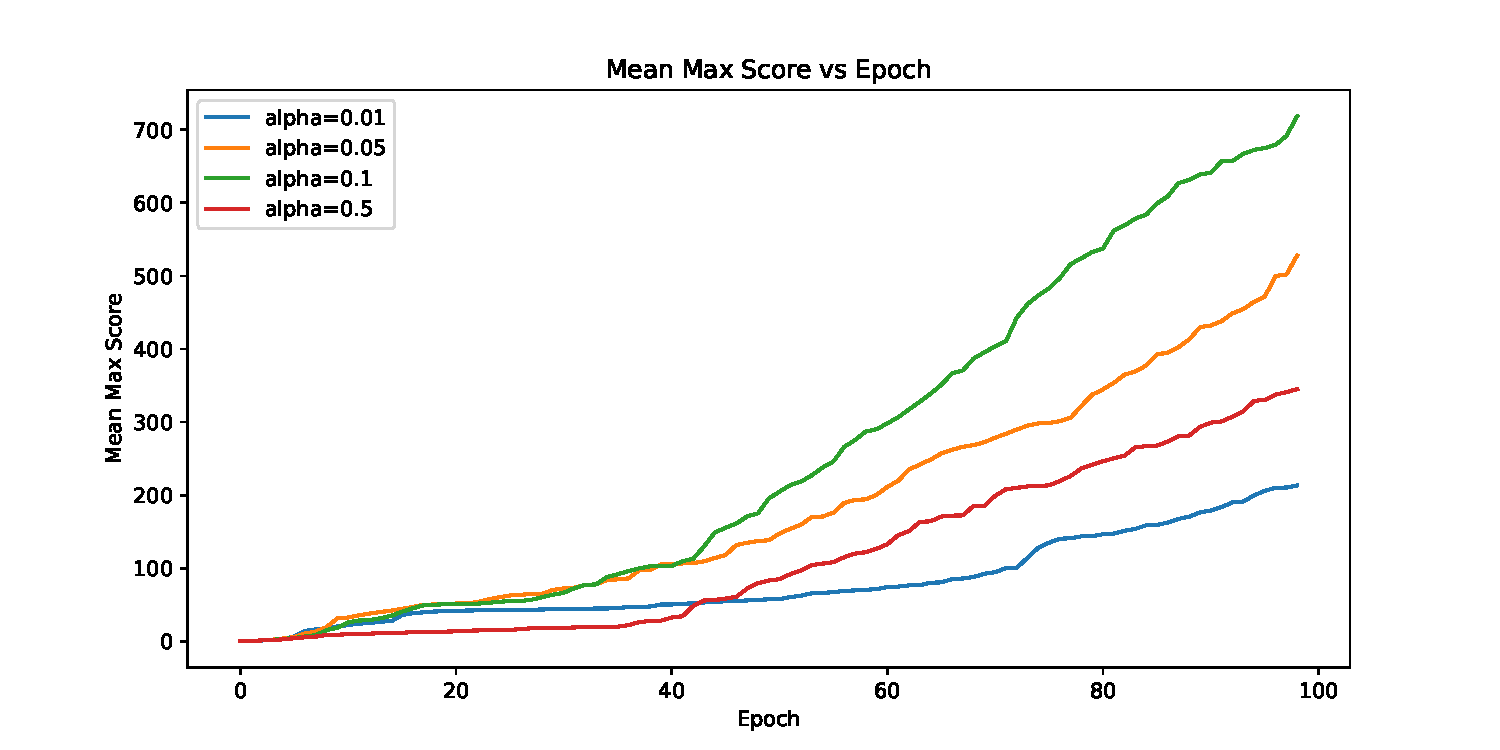
\includegraphics[scale=0.5]{figures/alpha_graph.pdf}
		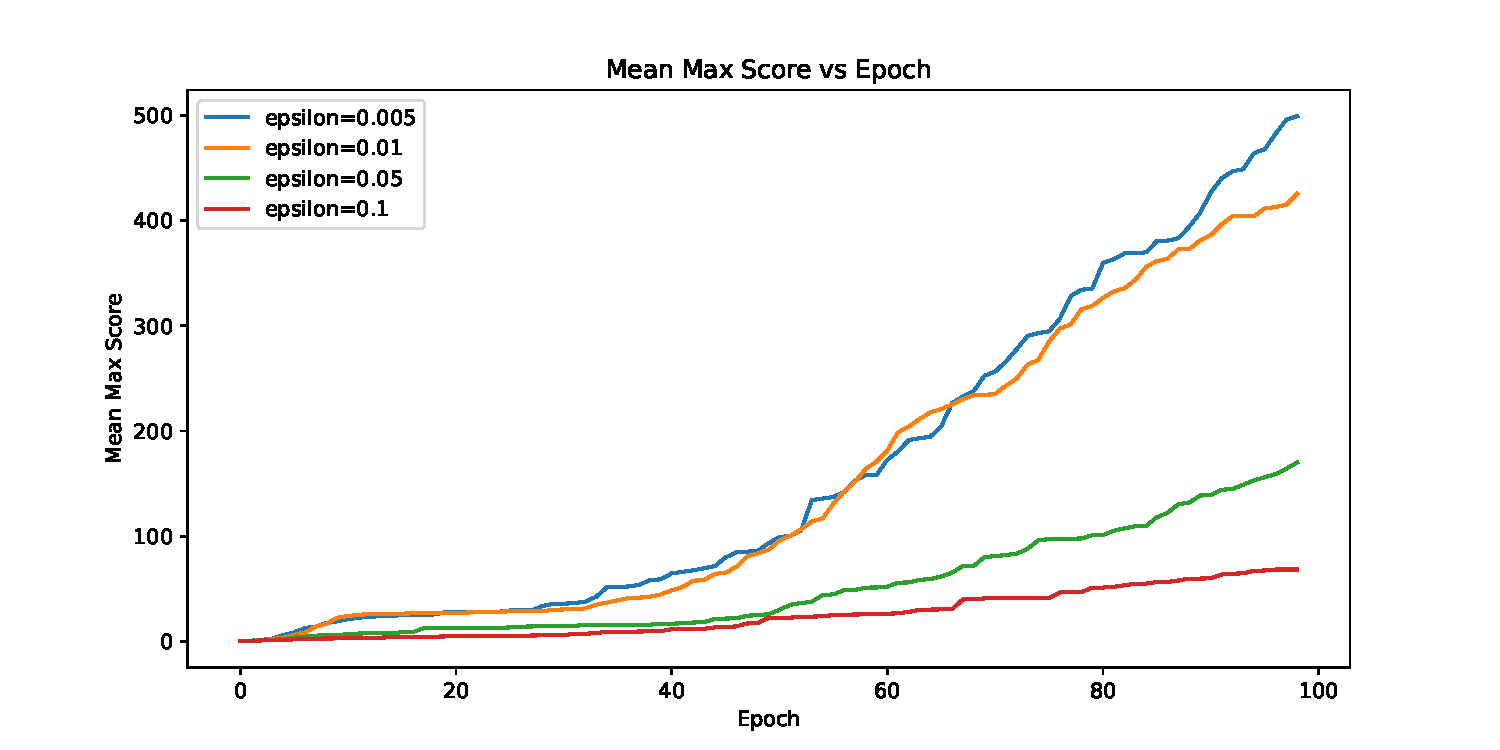
\includegraphics[scale=0.5]{figures/epsilon_graph.pdf}
	\end{center}


	Here is the code used to generate the data:
	\begin{minted}{python}
def mean_maxes(epsilon=0.01, alpha=0.5):
    epochs = 100

    hists = []
    for i in range(0, 100):
        agent = LearnerOptimized(epsilon=epsilon, alpha=alpha)
        hist = []
        run_games(agent, hist, epochs, 0)
        hists.append(hist)

    max_hists = [
        [max(hists[i][:n]) for n in range(1, epochs)] for i in range(0, len(hists))
    ]

    return [
        np.mean([max_hists[i][n] for i in range(0, len(hists))])
        for n in range(0, epochs - 1)
    ]
	\end{minted}
\end{parts}

\end{document}
